
\documentclass[12pt]{article}
\usepackage[a4paper, margin=.30in]{geometry}
\usepackage{graphicx ,
            wrapfig,
            xcolor, 
            enumerate,
            amsmath,
			fontenc,
			tcolorbox
            }

\newcommand\headerMe[2]{\noindent{}#1\hfill#2}
\renewcommand{\thesection}{\Roman{section}}

\author{Zakaria HAOUZAN}
\date{\today}

\begin{document}
% headers --------------
\headerMe{Matière : Physique-Chimie}{Professeur : Zakaria HAOUZAN}\\
\headerMe{Unité : Ondes }{Établissement : Lycée SKHOR qualifiant}\\
\headerMe{Niveau : 2BAC-SM-X}{Heure : 5H}\\

% ------Content ________
\begin{center}

    \Large{Leçon $N^{\circ} 3 $: \color{red}Propagation d'une onde lumineuse }
\end{center}
\section{Mise en évidence expérimentale de la diffraction de la lumière : }

\subsection{Expérience: }

Dans cette première expérience envoyonsàl'aide d'une source laser un faisceau lumineux étroit de longueur d'onde $\lambda = 633nm$ sur un écran.

On intercale entre l'écran et la source laser une plaque portant une fente de largeur a.
\begin{figure}[h]

	%\vspace{-1cm}
	\begin{center}
		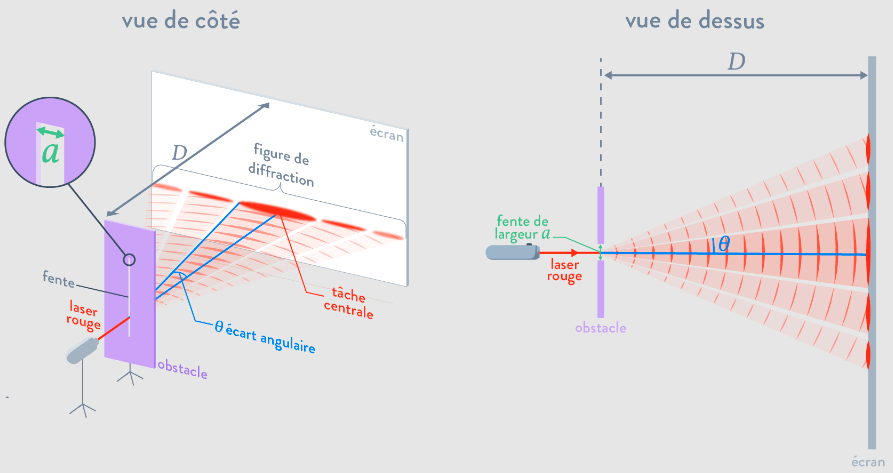
\includegraphics[width=0.9\textwidth]{./img/OLexperience.png}
	\end{center}
	\vspace{-1.5cm}
\end{figure}

\begin{itemize}
	\item Sur l'écran de projection situé à une distance D de la fente on observe une tâche centrale plus large entourée de part et
d'autres par des tâches secondaires moins larges et moins brillantes.

\item La fente se comporte comme une source lumineuse fictive, ce phénomène s'appelle diffraction de la lumière.
\end{itemize}


\begin{tcolorbox}
Remarque: 	
\begin{itemize}
	\item En remplaçant la fente par un obstacle très fin (un cheveu par exemple) on obtient les mêmes résultats que ceux trouvés
précédemment.

\item En utilisant une plaque contenant un trou circulaire, on obtient une tâche lumineuse circulaire entourée d'anneaux concentriques
d'intensité de plus en plus faible.

\item On constate expérimentalement que :
	\begin{itemize}
		\item La largeur de la tâche centrale augmente lorsque la largeur de la fente diminue.

		\item  La largeur de la tâche centrale augmente avec la longueur de l'onde lumineuse. (et aussi avec la distance D).
		\end{itemize}
	\end{itemize}
\end{tcolorbox}
\begin{figure}[h]
	\begin{center}
		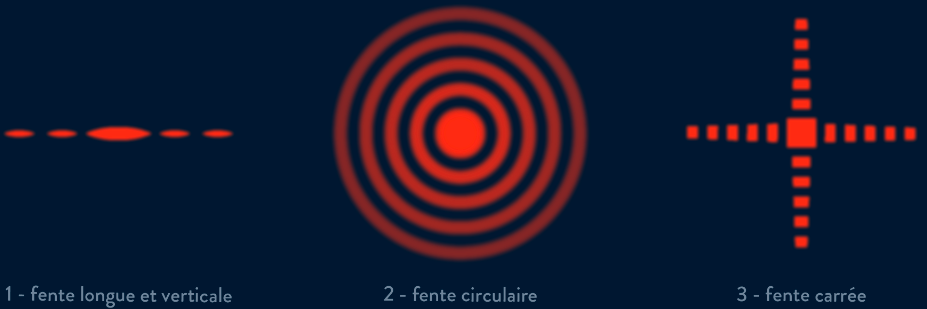
\includegraphics[width=0.9\textwidth]{./img/OLtypeDiff.png}
	\end{center}
	\vspace{-1.2cm}
\end{figure}
\subsection{Conclusion:}
\begin{tcolorbox}

Le phénomène de diffraction montre que la lumière a un aspect ondulatoire.

La lumière peut donc être caractérisée comme toutes les ondes, par sa célérité, sa fréquence et sa longueur d'onde.
\end{tcolorbox}
\begin{wrapfigure}[10]{r}{0.4\textwidth}
	\vspace{-1.5cm}
	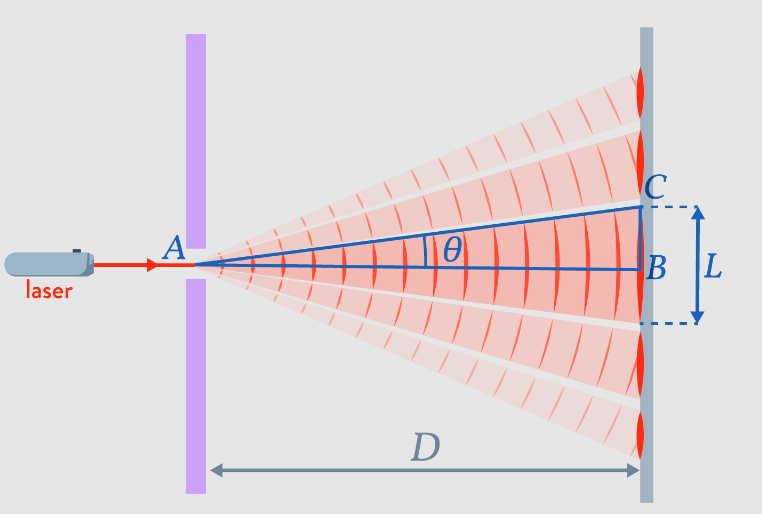
\includegraphics[width=0.4\textwidth]{./img/OLQngulaire.png}
\end{wrapfigure}
\subsection{Etude de la diffraction d'un faisceau laser par une fente:}
\subsubsection{L'écart angulaire:}

L'écart angulaire $\theta$ est l'angle sous lequel on voit la moitié de la tâches centrale depuis la fente de diffraction.
D'après la figure On a $$tan\theta = \frac{L}{2.D}$$ 

avec  : 

-L le largeur de la tâche centrale, en mètre (m);

-D la distance entre l’obstacle et l’écran, en mètre(m); 

Pour les angles petits $\theta$ mesurés en radian, on peut écrire :
	$tan\theta \approx \theta$   et $sin\theta \approx \theta$
	et $cos \theta \approx \theta$

	donc : $$\theta = \frac{L}{2.D} $$
	\subsubsection{Relation entre l'écart angulaire et la largeur de la fente: }

	\begin{wrapfigure}[0]{r}{0.4\textwidth}

	\vspace{2cm}
	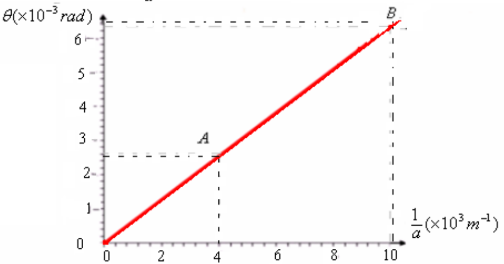
\includegraphics[width=0.4\textwidth]{./img/OLcourbe.png}

\end{wrapfigure}


	\section*{*Expérience:}
On pose l'écran à une distance D=1,5m puis on fait varier la largeur de la fente et on mesure dans chaque cas la largeur L de la tâche
centrale.
Tableau des résultats:
%\begin{center}

\begin{tabular}{ |c|c|c|c|c|c| }
	  \hline
	  a($\mu.m$) & 100 & 120 & 200 & 250 & 300  \\ \hline
	  L($mm$)	 & 19   &  15.8  & 9.5 & 7.6  & 6.3   \\\hline
	  $\theta$(x$10^{-3}rad$)& 6.33   & 5.26   & 3.17 & 2.53  & 2.1   \\\hline
	  $\frac{1}{a}$(x$10^{3}mm^{-1}$)	 & 10   &  8.33  &5  & 4  &3.33    \\\hline

\hline
\end{tabular}

%\end{center}
Représentation de la coube de variation de $\frac{1}{a}$ en fonction de $\theta$

On constate que $\theta$ est proportionnelle à, $\frac{1}{a}$ donc $\theta=K.\frac{1}{a}$

K:c'est le coefficient directeur de la droite qui représente $\theta$ en fonction de $\frac{1}{a}$.

\section*{le cocfficient directeur K : }
$$k = \frac{\Delta{\theta}}{\Delta{\frac{1}{a}}} = \frac{\theta_B - \theta_A}{(\frac{1}{a})_B -  (\frac{1}{a})_A} = \frac{(6.33 - 2.53).10^{-3}}{(10 - 4).10^3 m} = 633.10^{-9} = 633nm = \lambda$$

donc $$\theta = \frac{\lambda}{a}$$

\section*{Expression de la largeur de la fente: $\frac{\lambda}{a} = \frac{L}{2.D}$}
On constate expérimentalement que la largeur de la tâche augmente avec l'augmentation de D et de la longueur d'onde et elle diminue avec l'augmentation de la largeur (a) de la fente, ce qui est en accord avec les résultats de l'expérience.
\begin{tcolorbox}
Remarque:
	la diffraction par un trou circulaire de diamétre a, l'écart angulaire est donné par la relation suivante:$\theta$=$\frac{1.22.\lambda}{a}$.

	Dans le cas de la ditiraction par un fil de diamètre d, l'écart angulare est donné par la relation suivante $\theta = \frac{\lambda}{d}$
\end{tcolorbox}
	
\begin{wrapfigure}[0]{r}{0.4\textwidth}
	\vspace{-1cm}
	
\includegraphics[width=0.4\textwidth]{./img/OLapplication01.png}
\end{wrapfigure}
\section*{Exercice d'application 1: }
On réalise une expérience de diffraction , par un fil fin rectiligne , de la
lumière laser , de longueur d’onde $\lambda$. On observe , sur un écran l’image
ci-contre :
\begin{enumerate}
	\item Schématiser l’expérience en précisant l’orientation du fil .

	\item La figure de diffraction est la même que celle qui est donnée par une fente ayant une largeur égale au diamètre a du fil . Si D est la distance entre le fil et l’écran d’observation , et L la largeur de la tache centrale , quelle relation permet de déterminer $\lambda$ ? Préciser ces grandeurs sur le schéma .
 \item  Calculer $\lambda$

Données : $D = 7,70m$ ; $L = 2,0cm$ ; $a = 0,50mm$
\end{enumerate}

\section{Caractéristiques des ondes lumineuses : }
\subsection{Onde électromagnétique:}
La lumière n’est une onde mécanique, c’est une onde électromagnétique qui se propage dans les milieux transparents et dans le vide.
La vitesse de propagation de la lumière dans le vide (et dans l’air) est $c = 3.10^8m/s$ ( on l’appelle célérité).
\subsection{Lumière monochromatique et lumière polychromatique: }
\subsubsection{Lumière monochromatique : }
\begin{itemize}
	\item Toute radiation lumineuse ayant une seule couleur est dite monochro matique. Elle est caractérisée par sa fréquence $\nu$ qui ne change
pas avec le milieu de propagation .

\item Exemple :  laser est une source de lumière monochromatique cest-à-dire composée d'une seule radiation.
\item La longueur d'onde d'une lumière monochromatique dépend du milieu de propagation  $\lambda=\frac{v}{\nu}$.

\item La vitesse de propagation de la lumière dépend du milieu de propagation.
\item Exemples :La vitesse dans le vide et La vitesse  dans l'air : $c=3.10^8m/s$,La vitesse dans le verre $v_{verre}=2.10^8m/s$ , dans l'eau: $v_{eau}=2,25.10^8m/s$.
\end{itemize}

\begin{tcolorbox}
	Remarque: 
	La vitesse de propagation de la lumière dans le vide est : $c= 3.10^8m/s$, par conséquence la relation précédente $\lambda_0 = \frac{c}{\nu}$ 

	avec $\lambda_0$ est la longueur de l'onde lumineuse dans le vide.
\end{tcolorbox}
\begin{wrapfigure}[7]{r}{0.5\textwidth}
	\vspace{-1.5cm}
	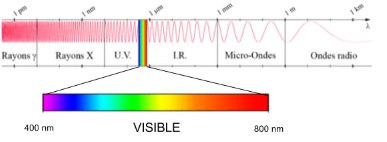
\includegraphics[width=0.5\textwidth]{./img/OLpolyChromatique.png}
\end{wrapfigure}

\subsubsection{lumière polychromatique : }

La lumière blanche (ou lumière visible ) est une lumière polychromatique composée de plusieurs radiations monochromatiques

Le mot polychromatique signifie composée de plusieurs couleurs .

Exemples : la lumière du soleil, celle de la lampe à incandescence ou de la bougie ...........

Le domaine de la lumière blanche (visible) est $400nm \leq \lambda \leq 800nm$ à l'extérieur de ce domaine de la lumière est invisible 
 
pour $\lambda \geq 800nm$ domaine de l'infrarouge

pour $\lambda \leq 400nm$ domaine de l'ultraviolet

\subsection{Indice de réfraction d'un milieu transparent : }

Chaque milieu transparent est caractérisé par son indice de réfraction qui est donné par la relation suivante:$$n = \frac{c}{v}$$

n:  indice de réfraction.

c: célérité de la umière dans le vide.

v:Vitesse de propagaton de la lumière dans le milieu.

Exemples : 

-l'indice de réfraction de l'air : $n_{air} = \frac{c}{v_{air}} = \frac{3.10^8}{3.10^8} = 1$

-l'indice de réfraction du verre : $n_{verre} = \frac{c}{v_{verre}} = \frac{3.10^8}{2.10^8} = 1.5$

-l'indice de réfraction de l'eau : $n_{eau} = \frac{c}{v_{air}} = \frac{3.10^8}{2.25.10^8} = 1.33$
\begin{tcolorbox}
	Remarque: Dans le vide on $c = \lambda_0.\nu$ Or dans un milieu donné : v = $\lambda.\nu$ donc $n = \frac{c}{v} = \frac{\lambda_0}{\lambda}$
\end{tcolorbox}

\subsection{Réfraction de la lumière :}
La réfraction de la lumière est le changement de direction que subi un rayon lumineux lorsqu'il passe d'un milieu transparent à un autre milieu
transparent.

\begin{figure}[h]
	\begin{center}

	\vspace{-0.5cm}
		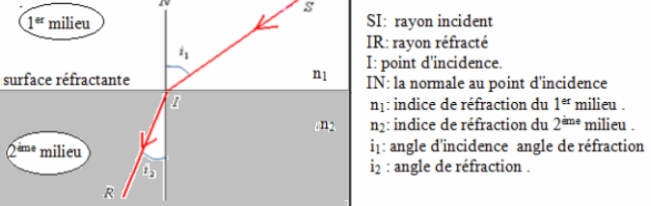
\includegraphics[width=0.7\textwidth]{./img/OLrefraction.png}
	\end{center}

	\vspace{-0.9cm}
\end{figure}
-Loi de Descartes de réfraction de la lumière: $n_1 sin(i_1) = n_2 sin(i_2)$ 2ème loi de réfaction

-Lorsque la lumière passe d'un milieu moins réfringent à un milieu plus réfringent $(n_2 \geq n_1)$ , le rayon réfracté s'approche de la normale.

-Lorsque la lumière passe d'un milieu plus réfringent à un milieu moins réfringent $(n_2 \leq n_1)$ , le rayon réfracté s'écarte de la normale.

\section*{Application 2: }
On envoie un faisceau de lumière de telle façon qu'il forme un angle de $70^{\circ}$ avec la surface de l'eau.

1.Sachant que l'indice de réfraction de l'air est $n_{air}=1$ et celui de l'eau est $n_{eau}=1,33$, déterminer la valeur de l'angle de réfraction.

2.Quelle sera la valeur de l'angle d'incidence si l'angle de réfraction est égal à $30^{\circ}$?

\begin{wrapfigure}[0]{r}{0.3\textwidth}
	\vspace{-2.8cm}
	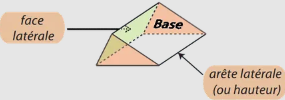
\includegraphics[width=0.3\textwidth]{./img/OLprisme.png}
\end{wrapfigure}


\section{Dispersion de la lumière: }
\subsection{Le prisme:}
Le prisme est un milieu transparent et homogène limité par deux faces planes non parallèles, la face opposée à l’arête est la base du
prisme.

\subsection{Trajet d'un faisceau lumineux à travers le prisme:}
On envoie un faisceau de lumière monochromatique sur la face d'un prisme, on constante que le faisceau subit une réfraction sur la
première face puis sur la deuxième face puis dévie vers la base du prisme.
\begin{figure}[h]
	\begin{center}

	\vspace{-0.5cm}
		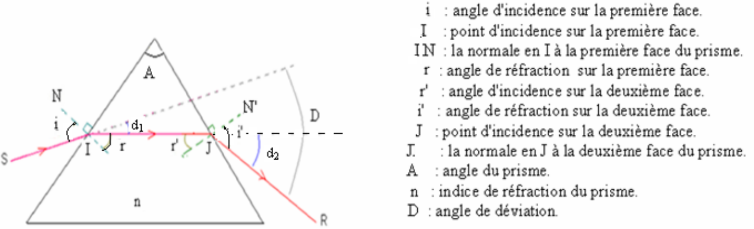
\includegraphics[width=0.8\textwidth]{./img/OLprismeCalc.png}
	\end{center}
	\vspace{-1.2cm}
\end{figure}

\subsection{Les relations du prisme: }

-Dans le triangle AIJ on a $A +(\frac{\pi}{2} - r) + (\frac{\pi}{2} - r') = \pi $ $\Rightarrow$ $A-r-r' = 0$ 

donc $$A=r+r'$$
En appliquant la loi de réfraction sur la première face du prisme: $sin i = n.sin r$

En appliquant la loi de réfraction sur la deuxième face du prisme: $nsin r' = sin i'$

L'angle de déviation: $D =d_1 + d_2$ = (i'-r') + (i-r) = i+i'-(r+r') = i+i'-A

donc $$D = i + i' -A $$
\begin{wrapfigure}[5]{r}{0.4\textwidth}
	\vspace{-1.2cm}
	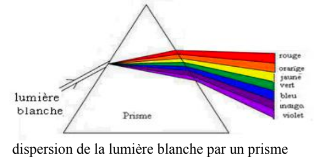
\includegraphics[width=0.4\textwidth]{./img/OLdispersionPrisme.png}
\end{wrapfigure}


\subsection{Dispersion de la lumière par un prisme: ++bonus++ }

Envoyons un faisceau de lumière blanche sur la première face d'un prisme, on obtient le spectre de la lumière blanche composé des
couleurs suivantes: rouge, orange, jaune, vert, bleu, indigo et violet.
Le prisme sépare les couleurs en les réfractant différemment cette décomposition de la lumière s'appelle dispersion.
\begin{itemize}
	\item La lumière blanche est composée d'un ensemble de lumières colorées appelées radiations.

	\item La dispersion de la lumière blanche par est due au fait que l'indice de réfaction du prisme dépend de la fréquence de l'onde lumineuse qui le traverse. 

	\item L'indice de rétraction d'un prisme est une fonction décroissante de la longueur de l'onde comme l'ndique
la relation de Cauchy  : $$n = a + \frac{b}{\lambda^2}$$
\begin{itemize}
	\item $\lambda$: La longueur de l'onde lumineuse.
	\item a et b sont des constantes.
	\end{itemize}
\item Par conséquence chaque radiation va subir une déviation diffèrente par le prisme ce qui entraine la dispersion de la lumière.
Donc le prisme est un milieu dispersif.

\end{itemize}

%*********************************************************************************************************
%\begin{wrapfigure}[10]{r}{0.5\textwidth}
%    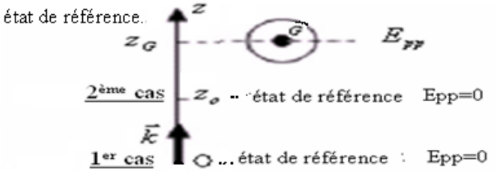
\includegraphics[width=0.5\textwidth]{./img/img00.png}
%\end{wrapfigure}


%\begin{figure}[h]
	%\begin{center}
		%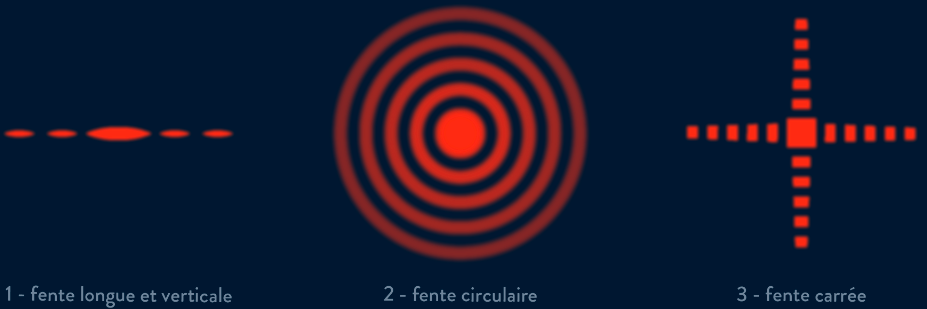
\includegraphics[width=0.9\textwidth]{./img/OLtypeDiff.png}
	%\end{center}
	%\vspace{-1.2cm}
%\end{figure}





%\begin{center}
   %\begin{tabular}{ |c|c|c|c|c|c|c| }
      %\hline
      %km & hm & dam & \bf{m} & dm & cm & mm \\
      %\hline
        %&   &    &  &   &   & \\
%\hline
%\end{tabular}
%On place un seul nombre dans chaque case.
%\end{center}
%\begin{center}
   %\begin{tabular}{ |c|c|c|c|c|c|c| }
      %\hline
      %$km^2$ & $hm^2$ & $dam^2$ & \bf{$m^2$} & $dm^2$ & $cm^2$ & $mm^2$ \\
      %\hline
        %&   &    &  &   &   & \\
%\hline
%\end{tabular}
%\end{center}


\end{document}

